\chapter{Use Cases \\
  \small{\textit{-- Evan Ciok, Sophia DiCuffa, Carson McManus, Cindy Lee}}
  \index{Chapter!use-cases}
  \label{Chapter::UseCases}}

There are a view different stakeholders with varying use cases:

\begin{itemize}
	\item Maintainer of OTT and OpenTogetherTube.com
	\item Self-hosted OTT instance administrator
	\item End users of OTT
\end{itemize}

\section{Use Case: Hosting the official website}

In this use case, the maintainer of OTT is hosting the official website, OpenTogetherTube.com. The website needs to remain deployable to Heroku, and the deployment pipelines need to continue to be functional.

\begin{figure}[!htb]
  \centering
  \scalebox{0.57}{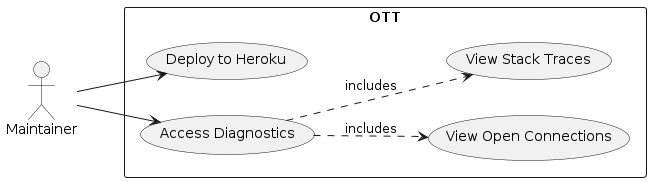
\includegraphics{Figures/use-case-maint.png}}
  \caption{\label{Figure::gossip-class-diaguse-case-maint} Use Case Diagram for Maintaining.}
\end{figure}


\section{Use Case: Self-hosting an instance of OTT}

In this use case, a user is hosting an instance of OTT on their own server. The user may or may not be using docker to deploy their instance. It should remain possible to deploy an instance of OTT without starting multiple services. Current deployments must continue to work when the user updates their instance of OTT.

\begin{figure}[!htb]
  \centering
  \scalebox{0.57}{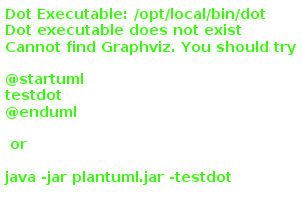
\includegraphics{Figures/use-case-self-host.png}}
  \caption{\label{Figure::gossip-class-diaguse-case-self-host} Use Case Diagram for Self Hosting.}
\end{figure}


\section{Use Case: Using any instance of OTT as an end user}

In this use case, an end user is using the website to watch videos. The end user must not see any difference between the current version of OTT and the new version of OTT with the load balancer. This implies that no changes to the client must be necessary.

\begin{figure}[!htb]
  \centering
  \scalebox{0.57}{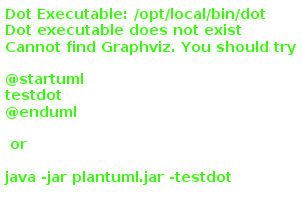
\includegraphics{Figures/enduser-usecase.png}}
  \caption{\label{Figure::enduser-usecase} Using OTT.}
\end{figure}